\documentclass{standalone}
\usepackage{tikz}
\begin{document}
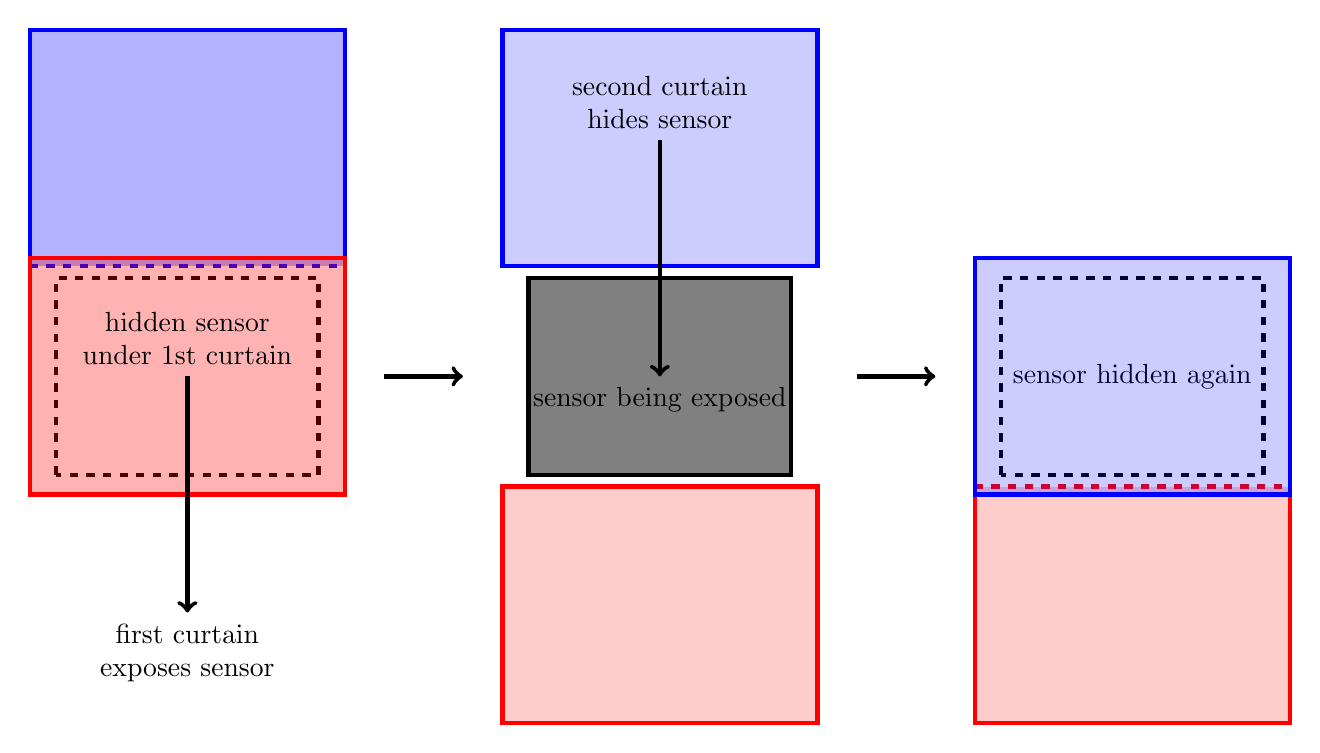
\begin{tikzpicture}

\def\sceneW{6cm}
\def\sceneWW{4.5cm}
\def\sceneSpace{1cm}
\def\planeW{4}
\def\planeH{3}
\def\planeSep{-0.1}
\def\backW{3.333}
\def\backH{2.5}
\def\backX{0.333}
\def\backY{0.25}
\def\clrfirst{red}
\def\clrsecond{blue}
\def\clrback{black}

\begin{scope}[ultra thick]
		% top overlap
		\draw [\clrsecond,dashed] (0,\planeH+\planeSep) -- ++(\planeW,0);
		%  _
		% | |
		\draw [\clrsecond,fill,fill opacity=0.3] (0,\planeH+\planeSep)
		      -- ++(0,\planeH) -- ++(\planeW,0) -- ++(0,-\planeH);
		% sensor
		\draw [\clrback,dashed] (\backX,\backY) rectangle ++(\backW, \backH);
		% bottom on sensor
		\draw [\clrfirst,fill=\clrfirst,fill opacity=0.3] (0,0) rectangle ++(\planeW,\planeH);

		% shutter move
		\draw [->] (0.5*\planeW,0.5*\planeH) node [align=center,above] {hidden sensor\\under 1st curtain} -- ++(0,-1.0*\planeH) node [align=center,below] {first curtain\\exposes sensor};
		% scene move
		\draw [->] (\sceneWW,0.5*\planeH) -- ++(\sceneSpace,0);

	\begin{scope}[xshift = \sceneW]
		% top still there
		\draw [\clrsecond,fill,fill opacity=0.2] (0,\planeH+\planeSep) rectangle ++(\planeW, \planeH);
		% shutter
		\draw [\clrback,fill=gray] (\backX,\backY) rectangle ++(\backW, \backH);
		% bottom has moved
		\draw [\clrfirst,fill,fill opacity=0.2] (0,-\planeH-\planeSep) rectangle ++(\planeW,\planeH);

		% shutter move
		\draw [->] (0.5*\planeW,1.5*\planeH) node [align=center, above] {second curtain\\hides sensor} -- ++(0,-1.0*\planeH) node [below] {sensor being exposed};
		% scene move
		\draw [->] (\sceneWW,0.5*\planeH) -- ++(\sceneSpace,0);
	\end{scope}

	\begin{scope}[xshift=2*\sceneW]
		%\draw [\clrfirst] (-\planeW-\planeSep,0) rectangle ++(\planeW,\planeH);

		% bottom is now under
		% bottom overlap
		\draw [\clrfirst,dashed] (0,-\planeSep) -- ++(\planeW,0);
		% |_|
		\draw [\clrfirst,fill,fill opacity=0.2] (0,-\planeSep)
		      -- ++(0,-\planeH) -- ++(\planeW,0) -- ++(0,\planeH);
		% sensor
		\draw [\clrback,dashed] (\backX,\backY) rectangle ++(\backW, \backH) node [align=center,pos=.5] {sensor hidden again};
		% top on sensor
		\draw [\clrsecond,fill,fill opacity=0.2] (0, 0) rectangle ++(\planeW, \planeH);
	\end{scope}

\end{scope}

\end{tikzpicture}
\end{document}
